\documentclass[a4paper,11pt]{article}

% ── Packages ──────────────────────────────────────────────────────────────────
\usepackage[
  a4paper,
  top=0.45cm,
  bottom=0.45cm,
  left=0.8cm,
  right=0.8cm
]{geometry}

\usepackage{fontspec}
\usepackage[sfdefault]{inter}      % Latin / numerals — Overleaf: TeX Live 2023+
\usepackage{xeCJK}                 % Japanese typesetting engine (compile with XeLaTeX)
\setCJKmainfont{Noto Sans CJK JP}  % swap for "Hiragino Kaku Gothic Pro" / "Yu Gothic" / "IPAexGothic" if unavailable
\setCJKsansfont{Noto Sans CJK JP}
\XeTeXlinebreaklocale "ja"
\XeTeXlinebreakskip = 0pt plus 1pt minus 0.1pt
\usepackage{textcase}
\usepackage{graphicx}
\usepackage{tikz}
\usepackage{fontawesome5}
\usepackage{array}
\usepackage{tabularx}
\usepackage{titlesec}
\usepackage{xcolor}
\usepackage{microtype}
\usepackage{hyperref}
\usepackage{enumitem}

\pagestyle{empty}
\setlength{\parindent}{0pt}

% ── Color Palette ─────────────────────────────────────────────────────────────
\definecolor{primaryblue}{RGB}{0, 75, 160}      % Deep professional blue
\definecolor{accentblue}{RGB}{0, 130, 220}     % Brighter blue for links/accents
\definecolor{darkgray}{RGB}{35, 35, 35}        % Primary body text
\definecolor{subtext}{RGB}{85, 85, 85}          % Metadata / Subtitles
\definecolor{rulecolor}{RGB}{200, 210, 225}     % Section dividers
\definecolor{lightbg}{RGB}{245, 247, 250}       % Photo background box

% ── Hyperlink Styling ────────────────────────────────────────────────────────
\hypersetup{
  colorlinks=true,
  urlcolor=accentblue,
  linkcolor=accentblue
}

% ── Section Styling ──────────────────────────────────────────────────────────
% (uppercasing is a Latin-only concept, so Japanese section titles pass through unchanged)
\titleformat{\section}
  {\Large\bfseries\color{primaryblue}}
  {}{0em}{}
  [\vspace{-10pt}{\color{primaryblue}\rule{\linewidth}{0.4pt}}\vspace{-2pt}]
\titlespacing*{\section}{0pt}{1pt}{-3pt}

% ── Table Alignment Helpers ──────────────────────────────────────────────────
\newcolumntype{L}{>{\raggedright\arraybackslash}p{2.6cm}}
\newcolumntype{G}{>{\raggedleft\arraybackslash}p{2.6cm}}
\renewcommand{\arraystretch}{1.08}

\newcommand{\role}[1]{{\itshape\color{subtext} #1}}
\newcommand{\meta}[1]{{\itshape\color{subtext} #1}}

% ── Document Start ───────────────────────────────────────────────────────────
\begin{document}
\color{darkgray}

% ── Header ────────────────────────────────────────────────────────────────────
\noindent
\begin{minipage}[c]{0.74\linewidth}
  {\fontsize{13}{15}\selectfont \textbf{\color{primaryblue}履歴書}}\\[1pt]
  {\fontsize{23}{27}\selectfont \textbf{\color{darkgray}Kartavya Suryawanshi}}\quad
  {\footnotesize\itshape\color{subtext}（カルタヴィヤ・スーリヤワンシー）}\\[4pt]
  \small
  \faMapMarker*\ 住所：IIT Mandi, Kamand, Himachal Pradesh, India\\[2pt]
  \faPhone\ 電話番号：+91 86689 44955
  \quad\textbullet\quad
  \faEnvelope\ メール：\href{mailto:b24199@students.iitmandi.ac.in}{b24199@students.iitmandi.ac.in}\\[2pt]
  \faLinkedin\ \href{https://www.linkedin.com/in/kartavya-suryawanshi-918753320/}{LinkedIn}
  \quad\textbullet\quad
  \faGithub\ \href{https://github.com/Kartavya728}{GitHub}\\[2pt]
  \textbf{生年月日：}2006年7月28日（満20歳）
  \quad\textbullet\quad
  \textbf{出身地：}インド・プネー
\end{minipage}%
\hfill
\begin{minipage}[c]{0.23\linewidth}
  \centering
  \begin{tikzpicture}
    % Shadow/Back Box
    \node[
      fill=primaryblue!15,
      minimum width=2.7cm,
      minimum height=2.7cm,
      rounded corners=4pt
    ] at (0.08,-0.08) {};
    % Main Frame Box
    \node[
      fill=lightbg,
      rounded corners=4pt,
      draw=primaryblue,
      line width=1.1pt,
      inner sep=1.5pt
    ] at (0,0) {
      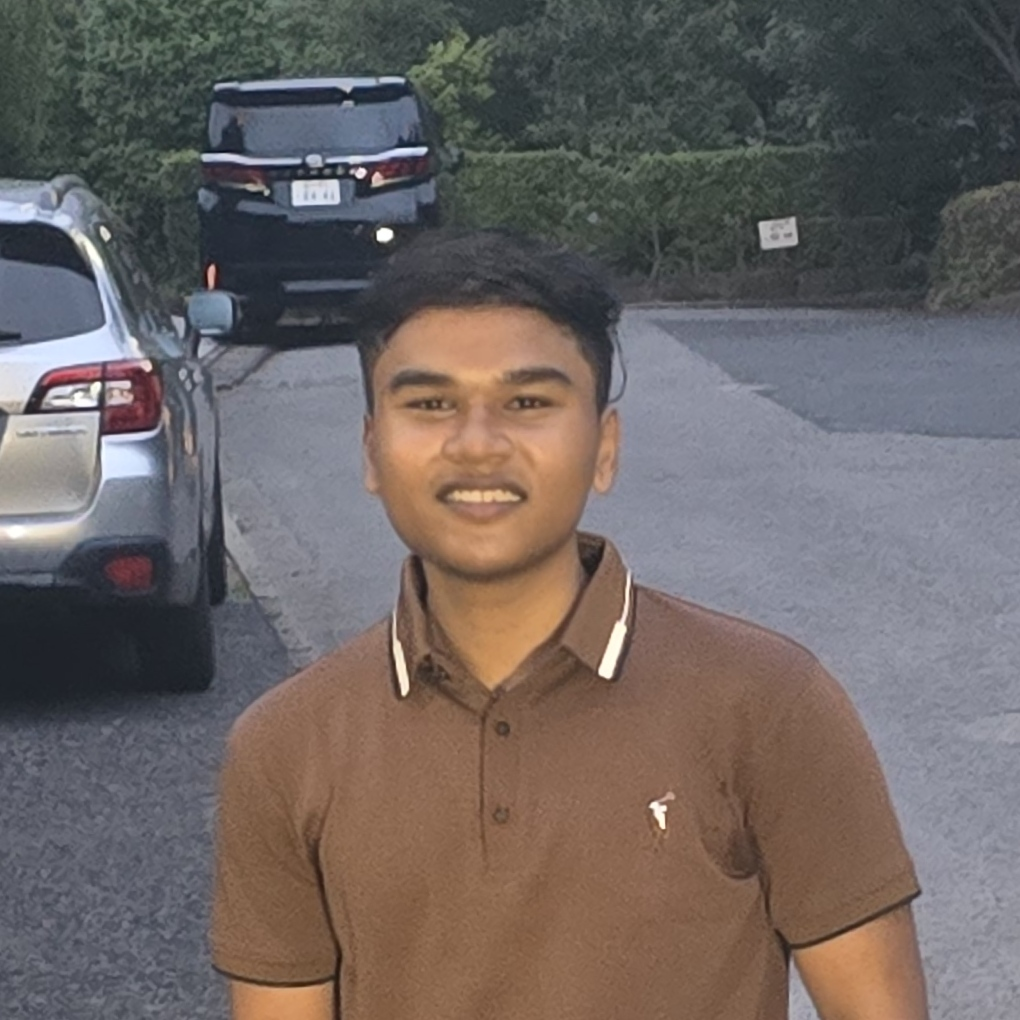
\includegraphics[width=2.6cm,height=2.6cm,keepaspectratio]{pro.jpeg}
    };
  \end{tikzpicture}
\end{minipage}

\vspace{2pt}
% Two-tone colored bar under header
\noindent
{\color{primaryblue}\rule{0.7\linewidth}{1.8pt}}{\color{accentblue}\rule{0.3\linewidth}{1.8pt}}
\vspace{-1pt}

% ── About Me / 自己PR ───────────────────────────────────────────────────────
\section*{自己PR}
\small
インド工科大学マンディ校（IIT Mandi）にてデータサイエンスを専攻する学部生です（\textbf{CGPA 9.27/10.0}）。機械学習・深層学習・フルスタック開発に強みを持ち、企業アナリティクスおよびWebエンジニアリングのインターンシップを通じて複雑な技術課題を実用的なソリューションへと落とし込んできました。全国規模のハッカソンで4度の優勝実績を持ち、スケーラブルなAIモデルと高性能データシステムの設計・構築に情熱を注いでいます。

% ── Higher Education ──────────────────────────────────────────────────────────
\section*{学歴（大学）}
\begin{tabularx}{\linewidth}{L X G}
  2024年 -- 現在 & \textbf{インド工科大学マンディ校（IIT Mandi）}、インド\newline
  \role{データサイエンス・エンジニアリング学科（DSE）　学士課程（B.Tech.）} & \textbf{\color{primaryblue}CGPA：9.27 / 10.0} \\[2pt]
  & \multicolumn{2}{p{15.4cm}}{\small\textbf{関連科目：}データ構造とアルゴリズム、機械学習、深層学習、行列計算、データ処理システム、線形代数、コンピュータ構成論}
\end{tabularx}

% ── School Education ──────────────────────────────────────────────────────────
\section*{学歴（中等教育）}
\begin{tabularx}{\linewidth}{L X G}
  2021年 -- 2023年 & \textbf{Jadhavar Jr.\ College}、プネー、マハーラーシュトラ州、インド\newline
  \role{高等学校卒業資格（12年生）　HSC教育委員会} & \textbf{86.0\%} \\[2pt]
  2016年 -- 2021年 & \textbf{NAJ Academy High School}、ムルド・ジャンジラ、マハーラーシュトラ州、インド\newline
  \role{中学校卒業資格（10年生）　SSC教育委員会} & \textbf{91.4\%}
\end{tabularx}

% ── Professional Experience ───────────────────────────────────────────────────
\section*{職務経歴}

\begin{tabularx}{\linewidth}{L X G}
  2026年6月 -- 2026年7月 &
  \textbf{野村不動産ホールディングス株式会社（Nomura Real Estate Holdings）}、東京、日本 \newline
  \role{データアナリティクス・インターン} & \\[-11pt]

  & \multicolumn{2}{p{15.4cm}}{\small
  \begin{itemize}[leftmargin=1.1em, topsep=0pt, itemsep=0pt, parsep=0pt]
    \item \textbf{Microsoft Viva Insights}を活用し、企業の生産性データを分析する\textbf{Power BI}自動ダッシュボードを構築。
    \item 統計分析によりワークフロー上のボトルネックを特定し、データドリブンな意思決定を支援。
  \end{itemize}} \\[1pt]

  2025年8月 -- 2025年12月 &
  \textbf{IIT Mandi 財務部（Finance Department）}、ヒマーチャル・プラデーシュ州、インド \newline
  \role{フルスタック・デベロッパー・インターン} & \\[-11pt]

  & \multicolumn{2}{p{15.4cm}}{\small
  \begin{itemize}[leftmargin=1.1em, topsep=0pt, itemsep=0pt, parsep=0pt]
    \item \textbf{React.js}、\textbf{Node.js}、\textbf{PostgreSQL}を用いた資金管理ポータルを開発。
    \item 助成金管理機能とロールベースアクセス制御（RBAC）を実装し、財務業務の効率化に貢献。
  \end{itemize}}
\end{tabularx}

% ── Achievements ──────────────────────────────────────────────────────────────
\section*{受賞歴・実績}
\small
\begin{tabularx}{\linewidth}{L X}
  2025年 & \textbf{優勝} --- \href{https://www.spaceappschallenge.org/}{NASA Space Apps Challenge}（参加100チーム以上中1位）：RAG（検索拡張生成）を活用した生命科学研究エンジン「\textit{Astrogenesis}」を開発。 \\[2.5pt]
  2025年 & \textbf{優勝} --- \href{https://www.ihub-data.iiit.ac.in/}{iHub Multimodal AIハッカソン}（参加1,600チーム以上中1位）：AI講義アシスタント「\textit{Smart Scribe}」の企画から実装まで一貫して開発をリード。 \\[2.5pt]
  2026年 & \textbf{優勝} --- \href{https://www.hcltech.com/}{Hack 60（HCLTech × IIT Mandi）}：ディープラーニング部門にて、リアルタイム・ディープフェイク検出および音声なりすまし防止システムにより1位を獲得。 \\[2.5pt]
  2026年 & \textbf{準優勝} --- \href{https://frosthack.com/}{Frosthack IIT Mandi}（参加50チーム以上中2位）：自律型マルチエージェントAIタスク・オーケストレーション・パイプラインを構築。
\end{tabularx}

% ── Skills ────────────────────────────────────────────────────────────────────

\section*{スキル}

\renewcommand{\arraystretch}{0.8}
\setlength{\tabcolsep}{3pt}

% NOTE: content cells are left unshifted (no \raisebox) so long bilingual
% skill lines can wrap naturally inside the X column instead of overflowing.
\newcommand{\skillcell}[1]{#1}

\begin{center}
\begin{tabularx}{\linewidth}{|>{\bfseries\color{primaryblue}}p{2.8cm}|X|}
\hline
プログラミング言語 &
\skillcell{C, C++, Python, JavaScript, TypeScript, HTML, CSS, SQL} \\ \hline

フレームワーク &
\skillcell{React.js, Next.js, Node.js, Express.js, Django, FastAPI, Tailwind CSS, LangChain, Streamlit} \\ \hline

AI・機械学習・深層学習 &
\skillcell{人工知能（AI）、機械学習（Machine Learning）、深層学習（Deep Learning）、PyTorch, TensorFlow, Scikit-learn, CNN, Transformer, オートエンコーダ, LLM, RAG} \\ \hline

クラウド・インフラ &
\skillcell{クラウドコンピューティング（Cloud Computing）, AWS, Git, Docker, Kubernetes, PostgreSQL, Supabase, Redis, MongoDB, Railway} \\ \hline

語学力 &
\skillcell{英語（C1相当）, 日本語（基礎レベル）, ヒンディー語, マラーティー語（母語）} \\ \hline

\end{tabularx}
\end{center}

\end{document}
